%- Quintile sorted predicted returns (simonian 2019)
%-OLS
% - summaries for coef attribution
%-RF
% - Summary for feat imp
% compare coefficients between feat imp and ols coef
% Sector rotation strat

\subsection{Hypothesis}

The aim of this subsection is to formalise ex ante hypotheses concerning the predictive accuracy and interpretability of all OLS and RF variations. 

We first consider the OLS base models. I speculate that within the estimation window, all factors in both the C4F and FF5 sets will attain statistical significance at the 5\% level when explaining monthly excess returns, yielding in\-sample $R^{2}$ values of at least 0.35.  This expectation is based on the well\-established risk\-pricing role of each factor: market excess return ($R_{M}-R_{f}$) as the primary driver per the Capital Asset Pricing Model, size ($SMB$) and value ($HML$) premia from \citeA{ff3_1993} foundational empirical findings, and the momentum effect ($UMD$) extended by \citeA{cahart_1997}. In the FF5 context, profitability ($RMW$) and investment ($CMA$) factors are likewise anticipated to be positively signed and signifitcant consistent with \citeA{novymarx_2013} Nevertheless, we expect the predictive $R^{2}$ out of sample to not be too low despite the inability of a static OLS framework to adapt to evolving market regimes (e.g.\ shifts in liquidity, sentiment, or sectoral leadership). An equity excess returns is usually not too wildly volatile (as we would see in section \ref{sec:data}), therefore it would not be too volatile to predict. %improve this in 2nd draft

%['vol', 'ret', 'shrout', 'prc', 'askhi', 'bidlo', 'put_volume','call_volume', 'put_call_ratio', 'vix_close', 'turn','zero_trade_ratio', 'baspread', 'mktrf', 'smb', 'hml', 'rmw', 'umd','cma', 'rf', 'enhanced_baker', 'news_sent', 'mktcap', 'turn_sd','sect_mktcap', 'mvel1', 'dolvol', 'daily_illq', 'excess_ret','excess_mkt_ret']

OLS enhanced models, due to possible multicollinearity among regressors inflating variance inflation factors and coefficients, I hypothesize that most of the Liquidity and Sentiment factors will remain statistically insignificant.  Consequently, I anticipate that only the original C4F factors (and market excess return in particular) will retain reliable significance, while overall in\-sample and out\-of\-sample $R^{2}$ will decline relative to the base OLS models. Therefore, OLS enhanced models is hypothesized to yield less accurate predictions.

The exceptionally turbulent market conditions of 2018 would exacerbate the limitations of linear OLS models, particularly in sectors such as Real Estate and Communication Services where idiosyncratic drivers dominate. In these conditions and certain segments, asset returns often exhibit behaviours that are macroeconomic dependent and nonlinear drawdowns that violate the constant-beta and homoskedasticity assumptions underlying OLS, which I hypothesize would yield biased forecasts and poor risk-adjusted performance. Consequently, while the expanded factor set may capture more risk dimensions, it is undermined by both linear model misspecification and the market conditions.

RF regression models offer a compelling non-parametric alternative to OLS by relaxing the linearity and additivity assumptions inherent in OLS. As an ensemble of decision trees, RF can capture nonlinear relationships and high order interactions among predictors without requiring an exact functional form. I therefore hypothesise that, when applied to monthly excess-return forecasting, RF will achieve both a higher in-sample $R^2$ and lower out-of-sample MSE than comparable OLS specifications. RF mitigates overfitting through bootstrap aggregation and random feature subsampling, so long as tuning parameters (tree depth, number of trees, minimum node size) are selected via cross-validation or out-of-bag error minimisation.

Nevertheless, the flexibility of RF does not guarantee uniform improvements across all forecasting Fama-French variations and enhancements. While RF inherently down weights irrelevant or redundant predictors through its random bootstrapping mechanism, deep trees can still split on spurious patterns or overfit if hyperparameters are poorly specified. We therefore anticipate that, under strict point forecast metrics or in macroeconomic situations that have low signal-to-noise ratio, an OLS model may outperform a naively tuned RF baseline. Still, for volatile and high growth sectors such as Real Estate where return drivers exhibit threshold effects, regime dependent nonlinearities, and intricate macro micro interactions RF's adaptive partitioning will yield substantial gains in predictive accuracy relative to linear models. Furthermore, due to the Random Forest specification, including a broad array of liquidity risk and sentiment proxies will not harm and even enhance RF's forecasting performance, in stark contrast to the coefficient instability induced by multicollinearity in OLS. Because each tree in the forest sees only a random subset of predictors at each split, correlated or redundant features are unlikely to dominate model variance, and the ensemble average remains stable. In terms of attribution, RF FI metrics (e.g., permutation importance or SHAP values) are expected to convey the same principal drivers of excess returns as OLS $t-statistics$, albeit without formal inferential guarantees such as confidence intervals or $p-values$. Thus, while RF output richer insights into interaction effects and nonlinear contributions, its interpretability must be framed in predictive terms

%todo: which Fama french variatio do you think will perfrom better, under which model?
\subsection{Model Interpretability: A Critique of pseudo-beta}

% - \citeA{simonian_2019} claimed that this could be a good substitute that could help communicate between machine learning models and finance people with a pseudo beta. However, with this data set and with the methods implemented, pseudo beta is unnlikely to be able to translate the findings of Random Forest into actual betas that are able to explain the returns of the assets.

% - It is found that, on all significant instance of any OLS coefficent of variables, RF is always off by 50\% or more. In some cases, we can see a 200 \% difference between the RF and OLS beta.

% - THerefore the notion of attempting to translate between RF betas and OLS is meaningless: This inconsistency goes against the notion of beta for financial experts: have a clear understanding of the drivers of returns and the ability to translate the findings of Random Forest into actual betas that are able to explain the drivers of the assets. Inconsistencies between these models muddy the water, and it does not have a statistical backing of t-tests.

% - However, though for attribution OLS is a better choice, for forecasting tools available are much more diverse and helpful. the magnitude of any variable effect could still be observed through SHAP, PDP and permutation importance so that finance professionals could still have a clear understanding of the drivers of returns.

\citeA{simonian_2019} originally proposed the concept of a “pseudo-beta” as a bridge between the predictive strengths of RF and the familiar beta coefficients derived from OLS, arguing that weighting RF variable importances by feature elasticity could yield interpretable analogues of linear factor loadings. However, when applied to our dataset and estimation procedures, the pseudo-beta approach fails to produce pseudo betas that are both numerically accurate and statistically reliable. Specifically, for every explanatory variable exhibiting a statistically significant OLS coefficient, the corresponding RF-derived pseudo-beta diverges from its OLS counterpart by at least 50\%, and in extreme cases by over 200\%. Such large discrepancies indicate that the pseudo-beta does not faithfully translate the nonlinear sensitivities learned by RF into the linear elasticity framework expected by financial practitioners. Therefore, OLS based factor models are still more appropriate to derive finance betas and answer questions such as "How many percent increase in excess returns can we expect if an increase in by 1\%?".

This inconsistency fundamentally undermines the utility of pseudo-beta as an interpretability tool: it contradicts the core financial utitlity that “beta” convey a stable measure of an asset's sensitivity to risk factors, complete with statistical rigor proof via $t$-tests. Instead of communicating with financial practicioners the drivers of returns, these unstable mappings only serve to “muddy the water” as the variability in pseudo-beta estimates lacks both statistical backing and economic coherence. Nonetheless, for forecasting applications, such as in this empirical study, practitioners are not without recourse. Model agnostic interpretability methods such as FI,SHAP values, partial dependence plots (PDP) and permutation importance can still reveal the relative magnitude and direction of each feature's impact on predicted returns. Below is a summary of the feature importances for each of the models, per sector.

Across the eleven GICS sectors, the RF baseline models display a strikingly uniform importance distribution. In both the C4F and FF5 variants, the excess-market return consistently absorbs the largest share of node split criterion weight (roughly 27-29\%). Size ($SMB$) and value ($HML$) follow at a respectful distance, while momentum ($UMD$) and, in the five-factor specification, profitability ($RMW$) and investment ($CMA$) divide the residual importance fairly evenly. The principal difference between \texttt{C4F} and \texttt{FF5} is minimal: the additional $RMW$ and $CMA$ factors only take a few percentage points from $MKT$, but no variable emerges as a clear new dominant driver. In short, factor contributions are not sector-specific in this analysis, nor does either factor set decisively outshine the other.

Once the models are enhanced with non-traditional predictors, a suprising shift occurs. The sentiment index of \citeA{wurgler_2007} claims close to 10 \% of total importance, displacing $MKT$ as the single most influential determinant of the forest's splits. By contrast, the two liquidity proxies (share turnover and the Amihud illiquidity ratio) exhibit negligible importance, suggesting that their information is either redundant with the traditional factors or consumed by the sentiment measure. Importantly, the inclusion of sentiment alters the importance without changing the uniformity of all the remaining factors. The traditional excess returns still share the bulk of explanatory power, but sentiment supplies an orthogonal source of predictability that the baseline models does not have access to. These findings imply that investor psychology is economically meaningful in sector-level return forecasting, whereas common liquidity metrics, though still share uniform weight in importance, adds less value in non-parametric models.

% For example, if finance practictioners want to look into what drives excess returns the Real Estate sector RF-EN-C4F model, they could look at SHAP values, Partial Dependence Plot (PDP) and Permutation Importance. 
% Automatically generated on 2025-06-29
            \begin{table}[ht]
            \centering
            \caption{\textit{Feature Importances by Sector for RF-BASELINE-C4F-ARL}}
            \label{tab:feature_importance_rf-baseline-c4f-arl}
            \begin{tabular}{lcccc}
            \toprule
            Sector & excess mkt ret & smb & hml & umd \\
            \midrule
            Communication Services & 0.281 & 0.239 & 0.240 & 0.240 \\\\
Consumer Discretionary & 0.281 & 0.237 & 0.243 & 0.238 \\\\
Consumer Staples & 0.287 & 0.238 & 0.237 & 0.238 \\\\
Energy & 0.274 & 0.240 & 0.241 & 0.246 \\\\
Financials & 0.263 & 0.227 & 0.268 & 0.242 \\\\
Health Care & 0.268 & 0.251 & 0.243 & 0.239 \\\\
Industrials & 0.279 & 0.243 & 0.233 & 0.245 \\\\
Information Technology & 0.288 & 0.229 & 0.240 & 0.243 \\\\
Materials & 0.278 & 0.244 & 0.234 & 0.244 \\\\
Real Estate & 0.276 & 0.236 & 0.250 & 0.238 \\\\
Utilities & 0.285 & 0.250 & 0.233 & 0.233 \\\\
            \bottomrule
            \end{tabular}%
            \end{table} 
% Automatically generated on 2025-06-26
            \begin{table}[H]
            \centering
            \caption{\textit{Feature Importances by Sector for RF-BASELINE-FF5-ARL}}
            \label{tab:feature_importance_rf-baseline-ff5-arl}
            \begin{tabular}{p{3.5cm}ccccc}
            \toprule
            Sector & \makebox[1.2cm]{excess mkt ret} & \makebox[0.8cm]{smb} & \makebox[0.8cm]{hml} & \makebox[0.8cm]{rmw} & \makebox[0.8cm]{cma} \\
            \midrule
            Communication Services & 0.235 & 0.198 & 0.199 & 0.189 & 0.179 \\\\
Consumer Discretionary & 0.235 & 0.194 & 0.202 & 0.190 & 0.178 \\\\
Consumer Staples & 0.230 & 0.188 & 0.187 & 0.214 & 0.182 \\\\
Energy & 0.235 & 0.206 & 0.215 & 0.178 & 0.166 \\\\
Financials & 0.236 & 0.189 & 0.252 & 0.164 & 0.158 \\\\
Health Care & 0.218 & 0.204 & 0.192 & 0.206 & 0.179 \\\\
Industrials & 0.237 & 0.200 & 0.204 & 0.191 & 0.168 \\\\
Information Technology & 0.236 & 0.190 & 0.184 & 0.203 & 0.188 \\\\
Materials & 0.234 & 0.206 & 0.202 & 0.190 & 0.168 \\\\
Real Estate & 0.242 & 0.202 & 0.232 & 0.166 & 0.158 \\\\
Utilities & 0.238 & 0.209 & 0.196 & 0.192 & 0.165 \\\\
            \bottomrule
            \end{tabular}%
            \end{table}
% Automatically generated on 2025-06-29
            \begin{table}[H]
            \centering
            \caption{\textit{Feature Importances by Sector for ENHANCED-RF-C4F-ARL (1)}}
            \label{tab:feature_importance_enhanced-rf-c4f-arl_1}
            \begin{tabular}{lcccccccc}
            \toprule
            Sector & \begin{tabular}[c]{@{}c@{}}excess mkt\\ret\end{tabular} & smb & hml & umd & turn & \begin{tabular}[c]{@{}c@{}}turn\\sd\end{tabular} & mvel1 & dolvol \\
            \midrule
            Communication Services & 0.084 & 0.076 & 0.080 & 0.075 & 0.078 & 0.000 & 0.075 & 0.064 \\\\
Consumer Discretionary & 0.084 & 0.075 & 0.077 & 0.078 & 0.079 & 0.000 & 0.084 & 0.063 \\\\
Consumer Staples & 0.094 & 0.074 & 0.072 & 0.074 & 0.074 & 0.000 & 0.075 & 0.071 \\\\
Energy & 0.084 & 0.075 & 0.073 & 0.079 & 0.099 & 0.000 & 0.068 & 0.077 \\\\
Financials & 0.078 & 0.069 & 0.080 & 0.076 & 0.106 & 0.000 & 0.090 & 0.068 \\\\
Health Care & 0.083 & 0.078 & 0.076 & 0.076 & 0.076 & 0.000 & 0.074 & 0.071 \\\\
Industrials & 0.085 & 0.076 & 0.075 & 0.074 & 0.077 & 0.000 & 0.086 & 0.066 \\\\
Information Technology & 0.090 & 0.076 & 0.079 & 0.078 & 0.072 & 0.000 & 0.072 & 0.068 \\\\
Materials & 0.084 & 0.080 & 0.076 & 0.077 & 0.075 & 0.000 & 0.080 & 0.068 \\\\
Real Estate & 0.090 & 0.078 & 0.079 & 0.073 & 0.103 & 0.000 & 0.087 & 0.048 \\\\
Utilities & 0.085 & 0.074 & 0.068 & 0.073 & 0.080 & 0.000 & 0.078 & 0.067 \\\\
            \bottomrule
            \end{tabular}%
            \end{table}
% Automatically generated on 2025-06-29
            \begin{table}[ht]
            \centering
            \caption{\textit{Feature Importances by Sector for ENHANCED-RF-C4F-ARL (2)}}
            \label{tab:feature_importance_enhanced-rf-c4f-arl_2}
            \begin{tabular}{lccccccc}
            \toprule
            Sector & daily illq & zero trade ratio & baspread & enhanced baker & vix close & put call ratio & news sent \\
            \midrule
            Communication Services & 0.070 & 0.000 & 0.068 & 0.052 & 0.132 & 0.068 & 0.077 \\\\
Consumer Discretionary & 0.065 & 0.000 & 0.065 & 0.050 & 0.124 & 0.075 & 0.081 \\\\
Consumer Staples & 0.071 & 0.000 & 0.098 & 0.056 & 0.108 & 0.067 & 0.066 \\\\
Energy & 0.062 & 0.001 & 0.081 & 0.049 & 0.111 & 0.064 & 0.077 \\\\
Financials & 0.057 & 0.005 & 0.085 & 0.040 & 0.105 & 0.064 & 0.076 \\\\
Health Care & 0.079 & 0.003 & 0.082 & 0.054 & 0.107 & 0.070 & 0.068 \\\\
Industrials & 0.066 & 0.001 & 0.072 & 0.049 & 0.124 & 0.067 & 0.081 \\\\
Information Technology & 0.069 & 0.001 & 0.079 & 0.053 & 0.114 & 0.076 & 0.073 \\\\
Materials & 0.068 & 0.000 & 0.078 & 0.052 & 0.114 & 0.068 & 0.081 \\\\
Real Estate & 0.061 & 0.000 & 0.068 & 0.046 & 0.129 & 0.069 & 0.068 \\\\
Utilities & 0.071 & 0.000 & 0.100 & 0.051 & 0.117 & 0.067 & 0.068 \\\\
            \bottomrule
            \end{tabular}%
            \end{table}
% Automatically generated on 2025-06-29
            \begin{table}[ht]
            \centering
            \caption{\textit{Feature Importances by Sector for ENHANCED-RF-FF5-ARL (1)}}
            \label{tab:feature_importance_enhanced-rf-ff5-arl_1}
            \begin{tabular}{lcccccccc}
            \toprule
            Sector & excess mkt ret & smb & hml & rmw & cma & turn & turn sd & mvel1 \\
            \midrule
            Communication Services & 0.081 & 0.074 & 0.073 & 0.068 & 0.066 & 0.070 & 0.000 & 0.069 \\\\
Consumer Discretionary & 0.077 & 0.068 & 0.071 & 0.074 & 0.067 & 0.073 & 0.000 & 0.077 \\\\
Consumer Staples & 0.079 & 0.067 & 0.066 & 0.087 & 0.068 & 0.071 & 0.000 & 0.068 \\\\
Energy & 0.081 & 0.073 & 0.069 & 0.065 & 0.059 & 0.086 & 0.000 & 0.067 \\\\
Financials & 0.077 & 0.064 & 0.079 & 0.059 & 0.059 & 0.102 & 0.000 & 0.080 \\\\
Health Care & 0.074 & 0.071 & 0.071 & 0.082 & 0.067 & 0.071 & 0.000 & 0.069 \\\\
Industrials & 0.080 & 0.070 & 0.066 & 0.070 & 0.063 & 0.071 & 0.000 & 0.080 \\\\
Information Technology & 0.087 & 0.071 & 0.068 & 0.085 & 0.075 & 0.066 & 0.000 & 0.064 \\\\
Materials & 0.076 & 0.079 & 0.069 & 0.074 & 0.064 & 0.067 & 0.000 & 0.073 \\\\
Real Estate & 0.089 & 0.067 & 0.085 & 0.066 & 0.059 & 0.095 & 0.000 & 0.085 \\\\
Utilities & 0.080 & 0.071 & 0.064 & 0.069 & 0.061 & 0.074 & 0.000 & 0.073 \\\\
            \bottomrule
            \end{tabular}%
            \end{table}
% Automatically generated on 2025-06-29
            \begin{table}[H]
            \centering
            \caption{\textit{Feature Importances by Sector for ENHANCED-RF-FF5-ARL (2)}}
            \label{tab:feature_importance_enhanced-rf-ff5-arl_2}
            \begin{tabular}{lcccccccc}
            \toprule
            Sector & dolvol & \begin{tabular}[c]{@{}c@{}}daily\\illq\end{tabular} & \begin{tabular}[c]{@{}c@{}}zero trade\\ratio\end{tabular} & baspread & \begin{tabular}[c]{@{}c@{}}enhanced\\baker\end{tabular} & \begin{tabular}[c]{@{}c@{}}vix\\close\end{tabular} & \begin{tabular}[c]{@{}c@{}}put call\\ratio\end{tabular} & \begin{tabular}[c]{@{}c@{}}news\\sent\end{tabular} \\
            \midrule
            Communication Services & 0.058 & 0.065 & 0.000 & 0.061 & 0.051 & 0.131 & 0.064 & 0.071 \\\\
Consumer Discretionary & 0.057 & 0.060 & 0.000 & 0.059 & 0.047 & 0.124 & 0.071 & 0.076 \\\\
Consumer Staples & 0.063 & 0.064 & 0.000 & 0.088 & 0.050 & 0.107 & 0.062 & 0.059 \\\\
Energy & 0.069 & 0.058 & 0.001 & 0.080 & 0.047 & 0.113 & 0.062 & 0.069 \\\\
Financials & 0.059 & 0.055 & 0.004 & 0.080 & 0.039 & 0.111 & 0.062 & 0.071 \\\\
Health Care & 0.068 & 0.070 & 0.003 & 0.077 & 0.048 & 0.104 & 0.064 & 0.062 \\\\
Industrials & 0.060 & 0.061 & 0.001 & 0.069 & 0.047 & 0.121 & 0.064 & 0.077 \\\\
Information Technology & 0.060 & 0.061 & 0.001 & 0.068 & 0.048 & 0.111 & 0.070 & 0.064 \\\\
Materials & 0.062 & 0.063 & 0.000 & 0.075 & 0.048 & 0.117 & 0.060 & 0.073 \\\\
Real Estate & 0.053 & 0.055 & 0.000 & 0.068 & 0.043 & 0.108 & 0.057 & 0.070 \\\\
Utilities & 0.059 & 0.066 & 0.000 & 0.094 & 0.047 & 0.116 & 0.061 & 0.063 \\\\
            \bottomrule
            \end{tabular}%
            \end{table}

\subsection{Model Performance Comparison}
\cref{tab:baseline_ols_c4f,tab:baseline_ols_ff5} reports the forecasting performance for the eight model specifications for each of the 11 sectors. The base OLS specifications provide only minimal explanatory power for daily sector level excess returns. In both the C4F and FF5 variants, the baseline models yield an in-sample $R^{2}$ below 1\%, confirming that a purely linear model cannot train on the nonlinear dynamics of almost 2 decades of the growing equity markets. Although the MSE and mean-absolute-error (MAE) values reported in  are numerically small, this is largely due to the low values of daily excess returns (typically the mean is  $<0.001\%$). Notably, for both the C4F and FF5 variants, the Financial sector (40) and especially Real Estate (60) has a high hold out MSEs (0.003 and 0.01 respectively). Augmenting the regressions with liquidity risks and sentiment factors  improves fit only marginally and Financial/Real Estate errors, while reduced, is still large. Overall, the enhanced OLS models remain vulnerable to market shifts and yield volatile out-of-sample errors, and the results show the limitations of linear factor models for forecasting.

By contrast, the RF frameworks deliver an immediate uplift in predictive accuracy. Even without the enhanced factors, the base RF models (\cref{tab:rf_baseline_c4f,tab:rf_baseline_ff5}) more than six fold the $R^{2}$ obtained with OLS and cut hold out (R)MSE by around 100\% on average. The gains are most striking for Real Estate, where RF achieves the second lowest sectoral hold out performace despite that sector's return volatility and liquidity. When liquidity and sentiment are incorporated (\cref{tab:enhanced_rf_c4f,tab:enhanced_rf_ff5}) the fit improves further, yet the incremental error reduction over the baseline RF is modest. This suggests that the tree ensemble already captures much of the nonlinear interaction between the traditional FF factors and the newly added variables. A contradicting pattern emerges across factor sets: the C4F specification excels in highly volatile sectors (notably 40 and 60), whereas FF5 produces a more uniform errors across the remaining segments. Taken together, these results confirm that RF creates a robust and generalisable foundation for the thesis's signal-generation and sector-rotation framework.

% Forecasting performance is of paramount importance in this thesis, as it forms the foundation of our signal creation process. Models must be robust across all market conditions, whether facing high liquidity risk, volatility, or shifts in sentiment, to effectively hedge against potential losses. \cref{tab:baseline_ols_c4f,tab:baseline_ols_ff5,tab:enhanced_ols_c4f,tab:enhanced_ols_ff5,tab:enhanced_rf_c4f,tab:enhanced_rf_ff5,tab:rf_baseline_c4f,tab:rf_baseline_ff5} present the forecasting performance metrics for each model specification and factor variation.

% - OLS Baseline: terrible fit (<1\% rsquared ). Though we see that the numerical values of mse, mae are quite tiny, we must remember that excess return is usually small below 0.001. Notably, for both c4f and ff5, sector 40 (fianncials) and especially 60 (real estate) did very poorly. Generally see no fitting for both Fama French variations with traditional OLS, but the RMSE hold indicates that they are not very robust in prediciting the 2018 hold out set. MAE does not tell us much due to it being very prone to outliers and this is a volatile hold out set.

% - OLS enahnced: fit improve only marginally for both FF variations, however still terrible. Sector 40,60 performance have improved but still moedls are very prone to errors.

% - RF base: Immediate significant imporvement in fit and in hould-out predictions. Surpring that sector 60, rf has the second lowest rmse hold out of all sector. Considering its volaitlity, this is massive win. One more surprise is that it seems like the more volatile the sector, the better the fit for C4F while it is the opposite for FF5, though this is marginal

% - RF enhanced:Significanf fit increase, comparing to base. Again, we see that c4f is performing better than ff5 on sector 40 and 60, ff5 is more stable across all sectors. However, interesting thing to note that the forecast prediction performance itself does not differ too much from base.

\subsection{Sector Rotation Strategy}
We evaluate the sector rotation strategy over a hold-out sample comprising the calendar year 2018. The strategy's performance is benchmarked against the S\&P500 returns index, which is weighted by market capitalization, computed as the product of share price and total shares outstanding. Many empirical studies benchmark their investment or sector rotation strategies against the S\&P500 due to its status as the primary large-cap U.S. equity market proxy, such as \citeA{sawar_2017} where the authors uses S\&P500 as a benchmark for a sector rotation strategy using FF5 alphas. As detailed in \cref{sec:data}, 2018 was characterized by heightened market volatility and adverse macroeconomic shocks; consequently, the cumulative return of the S\&P500 over this period was $-6.24\%$ \footnote{This paper omits the data point on 30-12-2018 since on 30/12/2018, there are no next day signal to be used for forecasting (next trading day is on 2019). Therefore the reported returns is different. If this data point is included, the cumulative return of the S\&P500 over this period was $-6.24\%$ indeed.}. The cummulative return of the equal-weighted portfolio is reported in \cref{tab:equal_weight} and \cref{fig:equal_weight_cum_ret_plot}. While the S\&P500 weighs every security based on their market capitalization, the equal-weighted portfolio assigns equal weight to each security, every trading day. It can be seen that a passive buy and hold equal-weighted portfolio, though operated at a loss in 2018, still beat the S\&P500 index by 4.79\%. This will be a common theme through out this results section. In 2018, due to market conditions, a negative returns does not mean that the strategy is performing poorly. However, if any strategy yields a positive return, it would be considered an outstanding performance by the model underlying that strategy.

\begin{figure}[H]
    \centering
    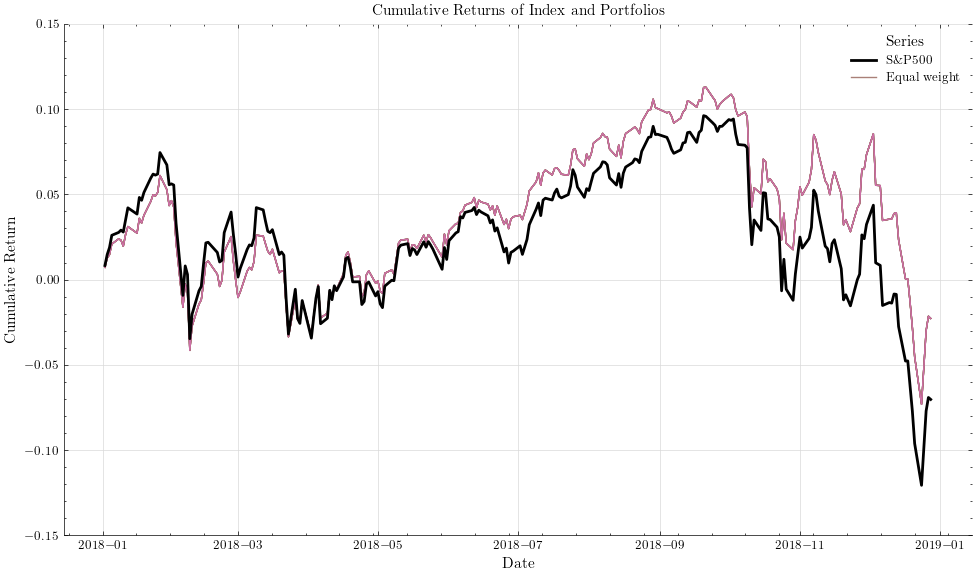
\includegraphics[width=\textwidth]{plots/results/equal_w_cum_ret_plot.png}
    \caption{Cumulative returns of S\&P500 and sector rotation strategies (2018)}\label{fig:eq_w_cum_ret_plot}
\end{figure}


\begin{table}[ht]
\centering
\caption{Descriptive Statistics of Index and Portfolio Returns}
\label{tab:return_stats_1}
\begin{tabular}{lrrrrrrr}
\toprule
{} & \multicolumn{1}{c}{Cumulative} & \multicolumn{1}{c}{Annualised} & \multicolumn{1}{c}{Annualised} & \multicolumn{1}{c}{Alpha} & \multicolumn{1}{c}{Information} & \multicolumn{1}{c}{PSR} & \multicolumn{1}{c}{PSR} \\
{} & \multicolumn{1}{c}{Return} & \multicolumn{1}{c}{Return} & \multicolumn{1}{c}{Volatility} & {} & \multicolumn{1}{c}{Ratio} & \multicolumn{1}{c}{(S*=0)} & \multicolumn{1}{c}{(S*=0.1)} \\
\midrule
S\&P500 & -7.03\% & -7.08\% & 17.06\% & 0.00\% & -- & -- & -- \\
equal\_weight & -2.27\% & -2.29\% & 15.39\% & 4.79\% & 0.29 & 0.92 & 0.45 \\
\bottomrule
\end{tabular}
\end{table}


To gauge risk-adjusted performance of the strategy, we report each portfolio's cumulative return, its active return relative to the S\&P500 (or 'Alpha'), and two spread sensitive statistics: the Information Ratio (IR) and the probabilistic Sharpe Ratio (PSR) at benchmark Sharpe thresholds $S^{*}=0$ and $S^{*}=0.1$. The IR evaluates excess return per unit of tracking-error volatility,

\begin{equation}
\mathrm{IR}=\frac{\mathbb{E}\left[R_{p}-R_{b}\right]}{\sigma\left(R_{p}-R_{b}\right)},
\end{equation}

where $R_{p}$ and $R_{b}$ are portfolio and benchmark returns, respectively, and a higher value signals more efficient investment relative to the risk taken by the investor. For example, an IR of below 0.1 means the strategy generates less than 0.1 units of excess return per unit of tracking error volatility, signaling that its returns are too small relative to their risk to justify strategy implementation. The PSR estimates the posterior probability that the true Sharpe ratio of a strategy exceeds a user-defined benchmark $S^{*}$,

\begin{equation}
\mathrm{PSR}= \Phi\left[\frac{\left(\hat{S}-S^{*}\right)\sqrt{T-1}}{\sqrt{1-\hat{S}^{2}/2}}\right],
\end{equation}
with $\hat{S}$ the sample Sharpe, $T$ the number of observations, and $\Phi(\cdot)$ the standard-normal cdf. Following \citeA{simonian_2019}, we report the PSR at $S^{*}=0$ and $S^{*}=0.1$.


The cumulative return chart for the in \cref{fig:cum_ret_plot} together with the summary statistics in \cref{tab:unconstr} shows the effectiveness of the active unconstrained sector rotation strategies relative to a passive S\&P 500 benchmark buy and hold strategy. While the index declined by 7.03\% over 2018\footnote{Due to ommitted data on 30/12/2018, 2018 period ends on 29/12/2018.}, 7 out of 8 models specifications outperformed the S\&P500 index, and 4 out of 8 specifications made positive returns despite the market conditions. The plot further shows that these active portfolios not only outperformed during the steady upswing through September but also sucessfully adjusted to the sudden sell off and increased volatility from mid-October onward, thereby dampening the loss.

A closer inspection reveals three surprises. First, the top three performers are all RF specifications, yet the fourth-best is an OLS specification. RF-C4f-EN is the best specification, achieving a cumulative return of 5.19\%, translating into an alpha of 12.31\%, an IR of 0.29 and a PSR of 0.97 at the 0.0 Sharpe benchmark.  Second, among RF variants the base FF5 variant outperforms its liquidity and sentiment enhanced variant. Opposite to that, the base RF C4F variant yield negative returns and performed worse than the enhanced OLS FF5 variant, while its enhanced c4f version is the best performing model. Third,  the only portfolio that underperformed the index was the base OLS FF5 (-10.66\%), while its enhanced specification is the only OLS model that generates a postive return, which confirms that both the additional liquidity and sentiment factors are crucial when momentum is missing. Another interesting observation is the RF enhanced models that are C4F variants yield better than their FF5 counterpart. This is probably due to momentum having a particularly strong effect in the macroeconomic environment of 2018, and profitability and investment factors delivered little incremental information.

The constrained strategy,which its statistics are reported in \cref{tab:constr} and \cref{fig:constr_cum_ret_plot}, shows a much more conservative approach to sector weight attribution. Evidently, \cref{fig:constr_cum_ret_plot} shows a much more tight clustering around the S\&P 500, while the unconstrained strategy fans out more. We could see in \cref{tab:constr} that, as expected,the order of the model performance stays exactly the same as the unconstrained model. An advantage of this strategy is that even for OLS models that underperformed against the S\&P500 in unconstrained strategy, the constrained strategy still outperformed the index. Even OLS base FF5 models, which had an active return of -3.58\%, had a positive return of 1.55\% in the constrained strategy. Similarly, OLS base c4f received a bump in active return of 2.2\%, comparing to the unconstrained strategy. What is surprising is that OLS enhanced C4F got lower active returns in the unconstrained strategy (3.2\%), compared to a 4.57\% increase in active returns in the constrained strategy.However, with lower risks comes lower returns. With the top 4 models, the unconstrained strategy got anywhere from 3 to 5\% more active returns than the constrained strategy.

However, implementing these models in actual trading applications requires much more than looking at raw return percentages. Each winning specification shows an IR of only 0.2-0.3, meaning that for every unit of active risk the strategy earns merely 0.2 to 0.3 units of excess return. This level of IR is considered modest at best, since institutional managers typically seek IRs above 0.5 to justify the costs and capacity constraints of active rotation \cite{gratton_2025}. The probabilistic Sharpe ratio at $S^{*} = 0$  with values around 40-60\% implying low confidence that the true Sharpe is larger than zero. In practice, one would prefer PSRs above 90\% at the target Sharpe to ensure robustness against estimation error. It essentially tell investors how likely they will make a positive return relative to the risk taken. In this case, we cannot reject the hypothesis that the true Sharpe ratio is zero. This is understandable given the volatility profile of 2018, where it is extremely uncertain that there would be any positive returns for any strategy. When we refer to the descriptive statistics of 2018, we could see how risky the market is.  Further research, with more computational resources could extend these strategies on a longer horizon (for example, using hold out set of 2016-2018), to have a more accurate outlook on the performance of these underlying models in less volatile periods.



% - Incredible results. Looking at the fig we could see that almost all of  the active strategies are outperforming the buy and hold index strategy. First four models, in a year where Sp500 index loses 7.03%, our strategy were able to hedge against that and even made positive returns. Only one model out of 8 lost against the index
% - In the fig we see that even  the plunge from mid october and volatile times at the end of the year , our models adjusted to that extremely well and generate signals that could hedge against the liquidity risk and sentiment shift
% - Looking closer: top 3 models are rf specification, but extremely surprising that 4rth is ols. Looking deeper in the top 4, c4f enhanced performed best with the cummulative ret =5.19\%, achieving an active return of 12.31\% . surprising that c4f is on top not ff5 {WHY DO YOU THINK c4f is on top not ff5}. even more surprising is that rf_base ff5 seems to beat rf_enhanced_ff5. {WHY IS THIS THE CASE}, with 11.44 active return comapred to 10.65\% active return. Most surpirasing of all, however, is that the 4rth place is not rf but an ols model, specifically ols_en_ff5 {WHY IS THIS POSSIBLE?}

% - Bottom 4 models: rf_base_c4f lost money {WHY enhanced do so good but base lost?}. Contrary to the hypothesis, ols base models performed worse than the ols enhanced, specifically c4f >ff5. Ols_base ff5 is the only one that lost money {WHY?}



\begin{figure}[H]
    \centering
    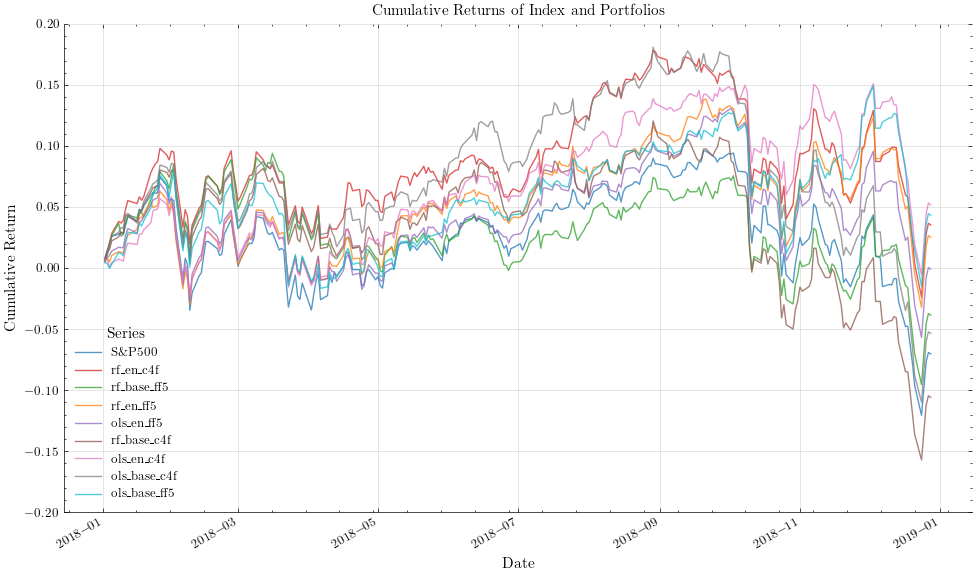
\includegraphics[width=\textwidth]{plots/results/cum_ret_plot.png}
    \caption{Cumulative returns of S\&P500 and sector rotation strategies (2018)}\label{fig:cum_ret_plot}
\end{figure}



% \begin{table}[ht]
% \centering
% \caption{Descriptive Statistics of Index and Portfolio Returns}
% \label{tab:unconstr}
% \begin{tabular}{lrrrrrrr}
% \toprule
% {} & \multicolumn{1}{c}{Cumulative} & \multicolumn{1}{c}{Annualised} & \multicolumn{1}{c}{Annualised} & \multicolumn{1}{c}{Alpha} & \multicolumn{1}{c}{Information} & \multicolumn{1}{c}{PSR} & \multicolumn{1}{c}{PSR} \\
% {} & \multicolumn{1}{c}{Return} & \multicolumn{1}{c}{Return} & \multicolumn{1}{c}{Volatility} & {} & \multicolumn{1}{c}{Ratio} & \multicolumn{1}{c}{(S*=0)} & \multicolumn{1}{c}{(S*=0.1)} \\
% \midrule
% S\&P500 & -7.03\% & -7.08\% & 17.06\% & 0.00\% & -- & -- & -- \\
% rf\_en\_c4f & 5.19\% & 5.23\% & 15.72\% & 12.31\% & 0.29 & 0.97 & 0.61 \\
% rf\_base\_ff5 & 4.33\% & 4.36\% & 16.45\% & 11.44\% & 0.28 & 0.95 & 0.57 \\
% rf\_en\_ff5 & 3.54\% & 3.57\% & 16.55\% & 10.65\% & 0.29 & 0.95 & 0.55 \\
% ols\_en\_ff5 & 2.53\% & 2.55\% & 16.27\% & 9.63\% & 0.28 & 0.95 & 0.53 \\
% rf\_base\_c4f & -0.08\% & -0.08\% & 16.10\% & 7.00\% & 0.26 & 0.93 & 0.48 \\
% ols\_en\_c4f & -3.85\% & -3.89\% & 16.48\% & 3.20\% & 0.22 & 0.89 & 0.38 \\
% ols\_base\_c4f & -5.34\% & -5.38\% & 17.23\% & 1.70\% & 0.21 & 0.86 & 0.33 \\
% ols\_base\_ff5 & -10.58\% & -10.66\% & 17.14\% & -3.58\% & 0.15 & 0.78 & 0.22 \\
% \bottomrule
% \end{tabular}
% \end{table}


% \begin{table}[ht]
% \centering
% \caption{Descriptive Statistics of Index and Portfolio Returns}
% \label{tab:constr}
% \begin{tabular}{lrrrrrrr}
% \toprule
% {} & \multicolumn{1}{c}{Cumulative} & \multicolumn{1}{c}{Annualised} & \multicolumn{1}{c}{Annualised} & \multicolumn{1}{c}{Alpha} & \multicolumn{1}{c}{Information} & \multicolumn{1}{c}{PSR} & \multicolumn{1}{c}{PSR} \\
% {} & \multicolumn{1}{c}{Return} & \multicolumn{1}{c}{Return} & \multicolumn{1}{c}{Volatility} & {} & \multicolumn{1}{c}{Ratio} & \multicolumn{1}{c}{(S*=0)} & \multicolumn{1}{c}{(S*=0.1)} \\
% \midrule
% S\&P500 & -7.03\% & -7.08\% & 17.06\% & 0.00\% & -- & -- & -- \\
% rf\_en\_c4f & -0.05\% & -0.05\% & 15.22\% & 7.03\% & 0.30 & 0.94 & 0.51 \\
% rf\_base\_ff5 & -0.29\% & -0.29\% & 15.39\% & 6.79\% & 0.30 & 0.93 & 0.50 \\
% rf\_en\_ff5 & -0.52\% & -0.53\% & 15.48\% & 6.55\% & 0.31 & 0.93 & 0.49 \\
% ols\_en\_ff5 & -0.83\% & -0.83\% & 15.45\% & 6.25\% & 0.30 & 0.93 & 0.48 \\
% rf\_base\_c4f & -1.59\% & -1.61\% & 15.42\% & 5.47\% & 0.29 & 0.92 & 0.46 \\
% ols\_en\_c4f & -2.71\% & -2.73\% & 15.43\% & 4.35\% & 0.27 & 0.91 & 0.43 \\
% ols\_base\_c4f & -3.16\% & -3.18\% & 15.66\% & 3.90\% & 0.27 & 0.91 & 0.42 \\
% ols\_base\_ff5 & -4.80\% & -4.84\% & 15.65\% & 2.24\% & 0.23 & 0.89 & 0.37 \\
% \bottomrule
% \end{tabular}
% \end{table}

%NEWWWWWWWWWWWWWWWW
\begin{table}[H]
\centering
\caption{Index and Portfolio Returns: Unconstrained Strategy}
\label{tab:unconstr}
\begin{tabular}{lrrrrrrr}
\toprule
{} & \multicolumn{1}{c}{Cumulative} & \multicolumn{1}{c}{Annualised} & \multicolumn{1}{c}{Annualised} & \multicolumn{1}{c}{Alpha} & \multicolumn{1}{c}{Information} & \multicolumn{1}{c}{PSR} & \multicolumn{1}{c}{PSR} \\
{} & \multicolumn{1}{c}{Return} & \multicolumn{1}{c}{Return} & \multicolumn{1}{c}{Volatility} & {} & \multicolumn{1}{c}{Ratio} & \multicolumn{1}{c}{(S*=0)} & \multicolumn{1}{c}{(S*=0.1)} \\
\midrule
S\&P500 & -7.03\% & -7.08\% & 17.06\% & 0.00\% & -- & -- & -- \\
rf\_en\_c4f & 5.19\% & 5.23\% & 15.72\% & 12.31\% & 0.29 & 0.61 & 0.10 \\
rf\_base\_ff5 & 4.33\% & 4.36\% & 16.45\% & 11.44\% & 0.28 & 0.59 & 0.09 \\
rf\_en\_ff5 & 3.54\% & 3.57\% & 16.55\% & 10.65\% & 0.29 & 0.57 & 0.08 \\
ols\_en\_ff5 & 2.53\% & 2.55\% & 16.27\% & 9.63\% & 0.28 & 0.55 & 0.07 \\
rf\_base\_c4f & -0.08\% & -0.08\% & 16.10\% & 7.00\% & 0.26 & 0.49 & 0.05 \\
ols\_en\_c4f & -3.85\% & -3.89\% & 16.48\% & 3.20\% & 0.22 & 0.40 & 0.03 \\
ols\_base\_c4f & -5.34\% & -5.38\% & 17.23\% & 1.70\% & 0.21 & 0.37 & 0.03 \\
ols\_base\_ff5 & -10.58\% & -10.66\% & 17.14\% & -3.58\% & 0.15 & 0.25 & 0.01 \\
\bottomrule
\end{tabular}
\end{table}

\begin{figure}[H]
    \centering
    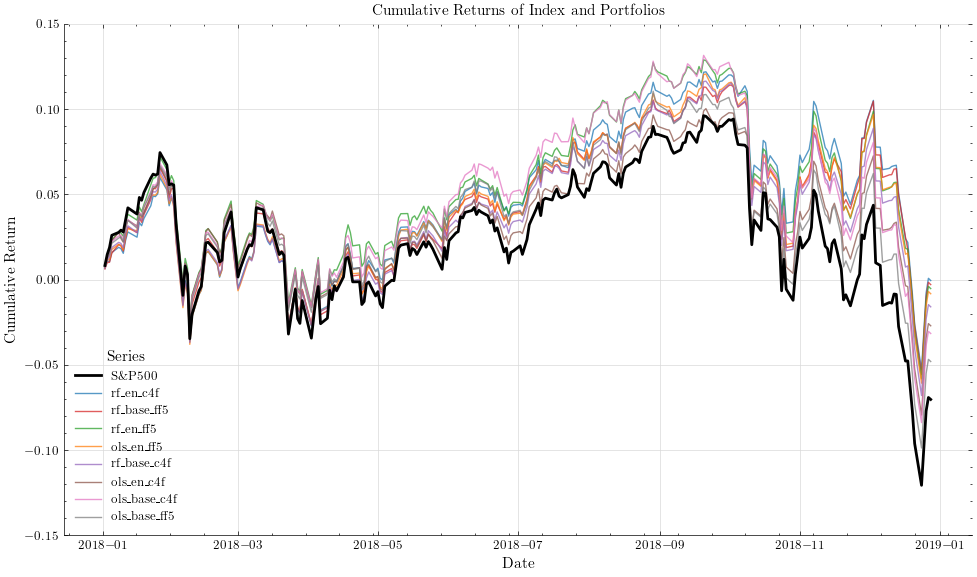
\includegraphics[width=\textwidth]{plots/results/contrained_cum_ret_plot.png}
    \caption{Cumulative returns of S\&P500 and sector rotation strategies (2018)}\label{fig:constr_cum_ret_plot}
\end{figure}

\begin{table}[H]
\centering
\caption{Index and Portfolio Returns: Constrained Strategy}
\label{tab:constr}
\begin{tabular}{lrrrrrrr}
\toprule
{} & \multicolumn{1}{c}{Cumulative} & \multicolumn{1}{c}{Annualised} & \multicolumn{1}{c}{Annualised} & \multicolumn{1}{c}{Alpha} & \multicolumn{1}{c}{Information} & \multicolumn{1}{c}{PSR} & \multicolumn{1}{c}{PSR} \\
{} & \multicolumn{1}{c}{Return} & \multicolumn{1}{c}{Return} & \multicolumn{1}{c}{Volatility} & {} & \multicolumn{1}{c}{Ratio} & \multicolumn{1}{c}{(S*=0)} & \multicolumn{1}{c}{(S*=0.1)} \\
\midrule
S\&P500 & -7.03\% & -7.08\% & 17.06\% & 0.00\% & -- & -- & -- \\
rf\_en\_c4f & -0.05\% & -0.05\% & 15.22\% & 7.03\% & 0.30 & 0.48 & 0.05 \\
rf\_base\_ff5 & -0.29\% & -0.29\% & 15.39\% & 6.79\% & 0.30 & 0.48 & 0.05 \\
rf\_en\_ff5 & -0.52\% & -0.53\% & 15.48\% & 6.55\% & 0.31 & 0.47 & 0.05 \\
ols\_en\_ff5 & -0.83\% & -0.83\% & 15.45\% & 6.25\% & 0.30 & 0.46 & 0.05 \\
rf\_base\_c4f & -1.59\% & -1.61\% & 15.42\% & 5.47\% & 0.29 & 0.44 & 0.04 \\
ols\_en\_c4f & -2.71\% & -2.73\% & 15.43\% & 4.35\% & 0.27 & 0.41 & 0.04 \\
ols\_base\_c4f & -3.16\% & -3.18\% & 15.66\% & 3.90\% & 0.27 & 0.40 & 0.03 \\
ols\_base\_ff5 & -4.80\% & -4.84\% & 15.65\% & 2.24\% & 0.23 & 0.36 & 0.03 \\
\bottomrule
\end{tabular}
\end{table}

\subsection{Discussion}
\subsubsection{Research Questions}

% \begin{enumerate}
%     \item \textbf{Research question 1}\
%     \textit{Does augmenting established linear asset-pricing models with liquidity-risk and sentiment factors, estimated via Random Forests, yield significantly higher out-of-sample explanatory power while retaining interpretability?}
%     \item \textbf{Research question 2}\
%     \textit{Given such an RF-based enhanced factor model, can its forecasts be combined with association-rule learning to derive simple, transparent sector-rotation rules that outperform the S\&P 500 index?}
%     \end{enumerate}

% Research question 1: Does augmenting established linear asset-pricing models with liquidity-risk and sentiment factors, estimated via Random Forests, yield significantly higher out-of-sample explanatory power while retaining interpretability?
% - Including liquidity risk and sentiment factors with Random Forest do yield a significantly higher out-of-sample explanatory power, compare to the baseline linear OLS models. However, it did not yield significantly higher out-of-sample explanatory power, compare to the baseline RF models.
% - Interpretaility approaches , though robust, is not as useful and strong as OLS's approach for financial practitioners. Method suggested by \citeA{simonian_2019}, in this analysis, produces uncamparable results to OLS counter parts, less informative, and lack statistical significance. How ever we could still get there with various alternatives (feature importance, shap, permutation importance) to see effect of each Fama french, liquidity, and sentiment factors on excess returns.
The findings of this thesis partly support the first research question. Enhancing the baseline C4F and  FF5 specifications with liquidity proxies (e.g.\ bid-ask spread, turnover, $ILLQ$) and the time varying sentiment index of \citeA{ung_2024} increases the out-of-sample $R^{2}$ and reduces hold out set forecast errors relative to plain-vanilla OLS benchmarks.  The gains, however, disappear once we benchmark RF against its own variants. It appears the tree ensemble already captures the same non-linearities and that liquidity and sentiment does not seem to significantly add forecasting power to the nonparametric model. In terms of interpretability, global coefficients from OLS remain easier for financial practitioners and managers to digest than feature importances from RF. The pseudo-beta approach proposed by \citeA{simonian_2019} is not only unsuitable for this particular empirical research, it also lacks the statisitcal rigour to be considered a valid substitute. However, when the primary objective is accurate forecasting, model-agnostic interpretability techniques (such as feature importance measures, SHAP values, and partial dependence plots) can elucidate the key drivers of returns in non-parametric models.


% Research Question 2: Given such an RF-based factor model, can its forecasts be combined with association-rule learning to derive simple, transparent sector-rotation rules that outperform the S\&P 500 index?
% - Yes. In both constrained and unconstrained strateies, ARL using RF forecasted rule outperforms S\&P 500 index. Through an empirical test, though we cannot definitely say due to only one year of backtesting, the enhancement factors in random forest models will not harm the performance of the rule-based strategy. Including them is seems to always be better than not. No overfitting/underfitting problems in our dataset. One strong evidence is our enhanced RF models are among the top performing models in the sector rotation strategy. For non-parametric models and for trading purposes, it seems like C4F and FF5 choice entirely depends on macroeconomic factors. 

%todo: Diebold–Mariano maybe?

This paper's approach and its findings support the second research question. Both the unconstrained and turnover-constrained implementations beat the S\&P500 on total return during the 2018 out-of-sample window, with no signs of over- or under-fitting. The inclusion of liquidity and sentiment factors never degrades strategy performance and, in most cases, improves it. The enhanced variant consistently rank among the top performers in the sector rotation strategy. Finally, the relative merits of $C4F$ versus $FF5$ inputs appear to hinge on current macroeconomic conditions rather than on any inherent superiority of one factor set over the other.

In terms of explainability, the framework developed in this paper delivers both the predictive accuracy of non-parametric learners and the transparency afforded by model-agnostic interpretability methods and rule-based trading signals. On any trading day, an individual forecast can be decomposed into the ARL sector rotation rule that generated the signal. That rule itself can be further can be traced back to each allocation decision back to specific Fama-French, liquidity, and sentiment factors via FI rankings (e.g.\ permutation importance or SHAP values), ensuring that every component of the prediction pipeline remains auditable and economically interpretable.

Nevertheless, the evidence should be regarded as preliminary and purely empirical: (i) only a single-year walk-forward evaluation of the expanding-window scheme has been completed, whereas a 20-year rolling back-test is required for robust inference; and (ii) the manual ARL support/confidence thresholds can make the rule set unstable. Replacing ARL with \emph{RuleFit}—a sparse additive rule ensemble—would fuse forecasting and explainability in one algorithm, avoid arbitrary thresholds, and yield naturally interpretable sector signals.

\subsubsection{Limitations}
% - Though we implemented extending window, computing resources limitataitons does not allow me to do 2 decades backtest. Ideally, this analysis should be doen with a proper extending window: train for X numbers of days lookback-> test day after. Then extend window. THen repeat for 20 years. THis paper did do the extending window continous retraining with extending window frame of 1 training year for 20 years. However it is reported as out-of-bag score only. With only 1 year to test out the extending window, it is not ideal. However it got a proxy what the actual result would be.

% - Constraints of ARL: This rule based method is based on manual threshold. Something of recent research, like RuleFit would be better. We are doing RF+ARL -> signals. However Rulefit does not need to be combined with anything else. It could create rules directly as a feature of the algo. These re actual if-then rules, such as "if market return >alpha and turn<= beta and news_sent> gamma then excess_return = 10\%".

% - Cannot statisically proof that either C4F or FF5 is better. But does not seem to entirely matter to non parametric models as we could include both (for forecasting purposes) SHAP, PDP and Feature Importance are only informative, not statisical proofs.
Despite implementing an expanding-window scheme, our back-test remains confined to a single year of walk-forward evaluation due to computational constraints. Ideally, we would train on an initial lookback of $X$ trading days, test on the subsequent day, then extend the training window and repeat this process continuously over a 20-year period. While this paper reports out of bag performance for a one-year training frame across two decades, the absence of a full dataset rolling back test in our study limits the robustness of our conclusions. Our one year proxy, however, suggests that the expanding window approach would likely produce comparable results over a longer time frame.

The ARL relies on manually selected support and confidence thresholds, which may render the extracted “if-then” sector-rotation rules sensitive to arbitrary parameter choices. Recent advances—such as the \texttt{RuleFit} algorithm, which generate sparse, additive rule ensembles directly from the data without the need for external rule mining and threshold tuning. By integrating rule extraction into the learner itself, RuleFit produces concise, interpretable rules (e.g.\ \emph{if} market return $>$ $\alpha$ \emph{and} turnover $\le \beta$ \emph{and} sentiment $>$ $\gamma$, \emph{then} excess return $=10\%$) while avoiding the two-step RF+ARL pipeline.

Finally, we cannot statistically demonstrate that the C4F or FF5 formulations are superior within a non-parametric forecasting framework. In practice, RF models can accommodate both factor sets simultaneously and simply don't split on redudant predictors. Moreover, interpretability tools—feature importance, SHAP values, and PDP—offer descriptive insights into factor contributions but do not constitute formal hypothesis tests. Future work should incorporate inferential procedures (e.g.\ testing differences in out-of-sample $R^2$ or using bootstrap confidence intervals for SHAP contributions) to underpin the economic relevance of each factor choice.

\subsubsection{How investors and asset managers can use the findings of this paper}
% - ideal workflow: gather past data -> plug in -> auto feature engineers_> pipeline (rf -> arl-> rules) -> weighting on tomorrows sector. Tomorrow comes, automatcially include today in traning window, adjust for todays excess returns -> forecast tomorrow -> weight tomorrow..
% - When an actual trade is not as expected -> can go back and see exactly which factor caused the trade to be not as expected with feature importance, shap, pdp
% - With incorporation of sentiment, liquidity risks, can think about other macroeconomic factoers that are less niche, since the two most promonient factors are taken into account. Help financial professional make better decisions that are always explainable at every single step of the trading route
For asset managers, this is the proposed pipeline: automated data ingestion $\rightarrow$ feature engineering $\rightarrow$ RF forecasting $\rightarrow$ rule extraction. This pipeline delivers a daily sector-weight vector whose rationale can be traced factor-by-factor. When live trades deviate from expectations, global and local attribution via feature importance, SHAP, or partial dependence immediately isolates which of the traditional FF factors ($SMB$, $HML$, $MOM$, $RMW$, $CMA$), the liquidity variables, or the sentiment index drove the surprise deviation. Because liquidity risk and sentiment already proxy two of the most pervasive macro drivers, practitioners can next experiment with complementary state variables (e.g.\ term-structure slope, credit spreads) without materially inflating model complexity.


% \noindent\textbf{Recommended refinements and theoretical checks}
% \begin{itemize}
% \item \emph{Statistical testing}: report out-of-sample $\Delta R^{2}$ p-values and Diebold-Mariano statistics to demonstrate that RF-based enhancements are materially better than OLS and not materially worse than vanilla RF.
% \item \emph{Factor choice}: clarify why $C4F$ vs.\ $FF5$ matters once non-parametric learners are used; consider including both sets of factors and letting the algorithm down-weight redundant ones.
% \item \emph{Back-test design}: extend the expanding-window evaluation to the full 1990-2018 span; document walk-forward hyper-parameter tuning to avoid look-ahead bias.
% \item \emph{Interpretability caveat}: remind readers that SHAP and permutation scores are \emph{not} formal statistical betas; they measure marginal predictive contribution, not economic elasticity.
% \item \emph{Liquidity–sentiment theory}: verify that liquidity betas indeed earn a premium during market stress (e.g.\ 2008, 2020) and that sentiment loads interact with the size factor, as implied by \citeA{baker_wurgler_2007}.
% \end{itemize}